\section{Sigma-Delta Wandler}

\begin{multicols}{2}
	\paragraph{Zeitkontinuierliches Modell} ~\\
	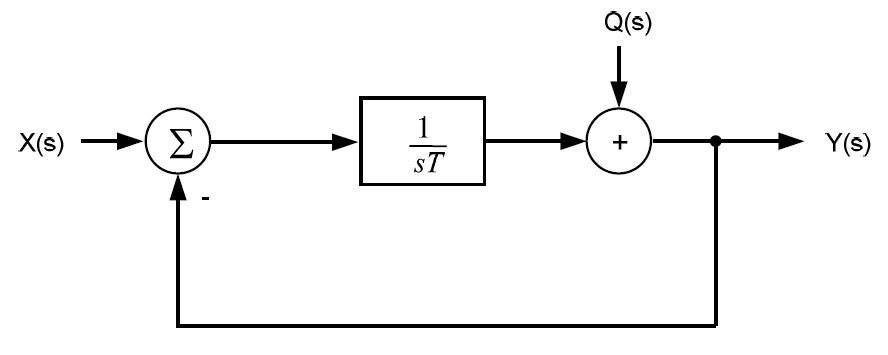
\includegraphics[width=0.8\linewidth]{images/sigma_delta.jpg}
	\begin{align*}
		\text{Signal UTF:} \quad & H_s(s) = \frac{1}{1+sT} \\
		\text{Noise UTF:} \quad & H_n(s) = \frac{sT}{1+sT}
	\end{align*}
	\vfill\columnbreak
	\paragraph{Zeitdiskretes Modell} ~\\
	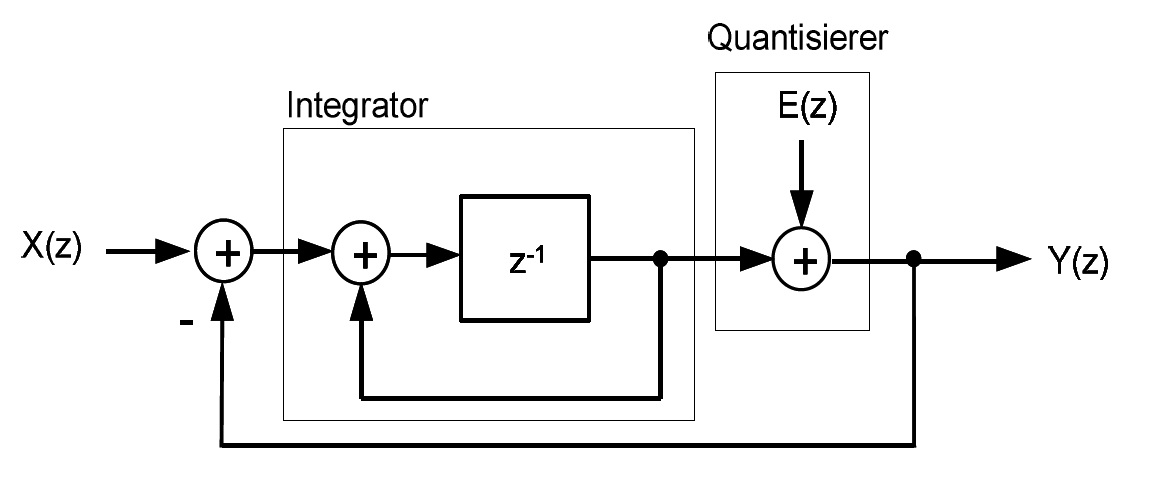
\includegraphics[width=0.8\linewidth]{images/sigma_delta_diskret.jpg}
	\begin{align*}
		\text{Signal UTF:} \quad & H_s(z) = z^{-1} \\
		\text{Noise UTF:} \quad & H_n(z) = 1-z^{-1}
	\end{align*}
\end{multicols}

\subsection{Pattern Noise}
DC-Eingangsspannungen führen zu repetitiven Sequenzen am Modulator-Ausgang, so genanntem Pattern Noise.
Ist $x$ sehr klein, entstehen repetitive Sequenzen tiefer Frequenz.
\begin{center}
	\begin{tabular}{ll}
		\textbf{Eingangsspannung} & \textbf{Pattern Noise Periode} \\ \hline
		$V_{\In} = 0$ & $\frac{1}{2} \Fclk$\\
		$V_{\In} = \pm \frac{1}{2} V_{\Ref}$ & $\frac{1}{4} \Fclk$ \\
		$V_{\In} = \pm \frac{1}{8} V_{\Ref}$ & $\frac{1}{16} \Fclk$ \\
		$V_{\In} = \pm 0.1 V_{\Ref}$ & $\frac{1}{20} \Fclk$ \\
		$V_{\In} = x \cdot V_{\Ref}$ & $\frac{x}{2} \Fclk$\\
		\hline
	\end{tabular}
\end{center}


\subsection{Signal-Rausch-Abstand}

Für einen $n$-bit Modulator bei einer Signalfrequenz von $f_0$ kann das Rauschen wie folgt berechnet werden:
\begin{flalign*}
	&\text{Signal-to-Noise Ratio} && \text{SNR} && \approx -3.4 + 6 n + 9 \log_2\left(OSR\right) \\
	&\text{Oversampling Ratio} && \text{OSR} && = \frac{f_s / 2}{f_0} \\
	&\text{Effektivwert $n_0$ der Rausch-Spannung für Ordnung $n=1$} && n_0 && \approx \frac{q}{\sqrt{12}} \frac{\pi}{\sqrt{3}} \left(\frac{2 f_0}{f_s}\right)^{3/2} \\
	&\text{Effektivwert $n_0$ der Rausch-Spannung für Ordnung $n=2$} && n_0 && \approx \frac{q}{\sqrt{12}} \frac{\pi^2}{\sqrt{5}} \left(\frac{2 f_0}{f_s}\right)^{5/2} \\
	&\text{Effektivwert $n_0$ der Rausch-Spannung für Ordnung $n=3$} && n_0 && \approx \frac{q}{\sqrt{12}} \frac{\pi^3}{\sqrt{7}} \left(\frac{2 f_0}{f_s}\right)^{7/2} \\
\end{flalign*}